\documentclass[tikz,border=10pt]{standalone}
\usepackage{tikz}
\usetikzlibrary{positioning, arrows.meta, shapes.geometric, fit, backgrounds, calc}

\begin{document}
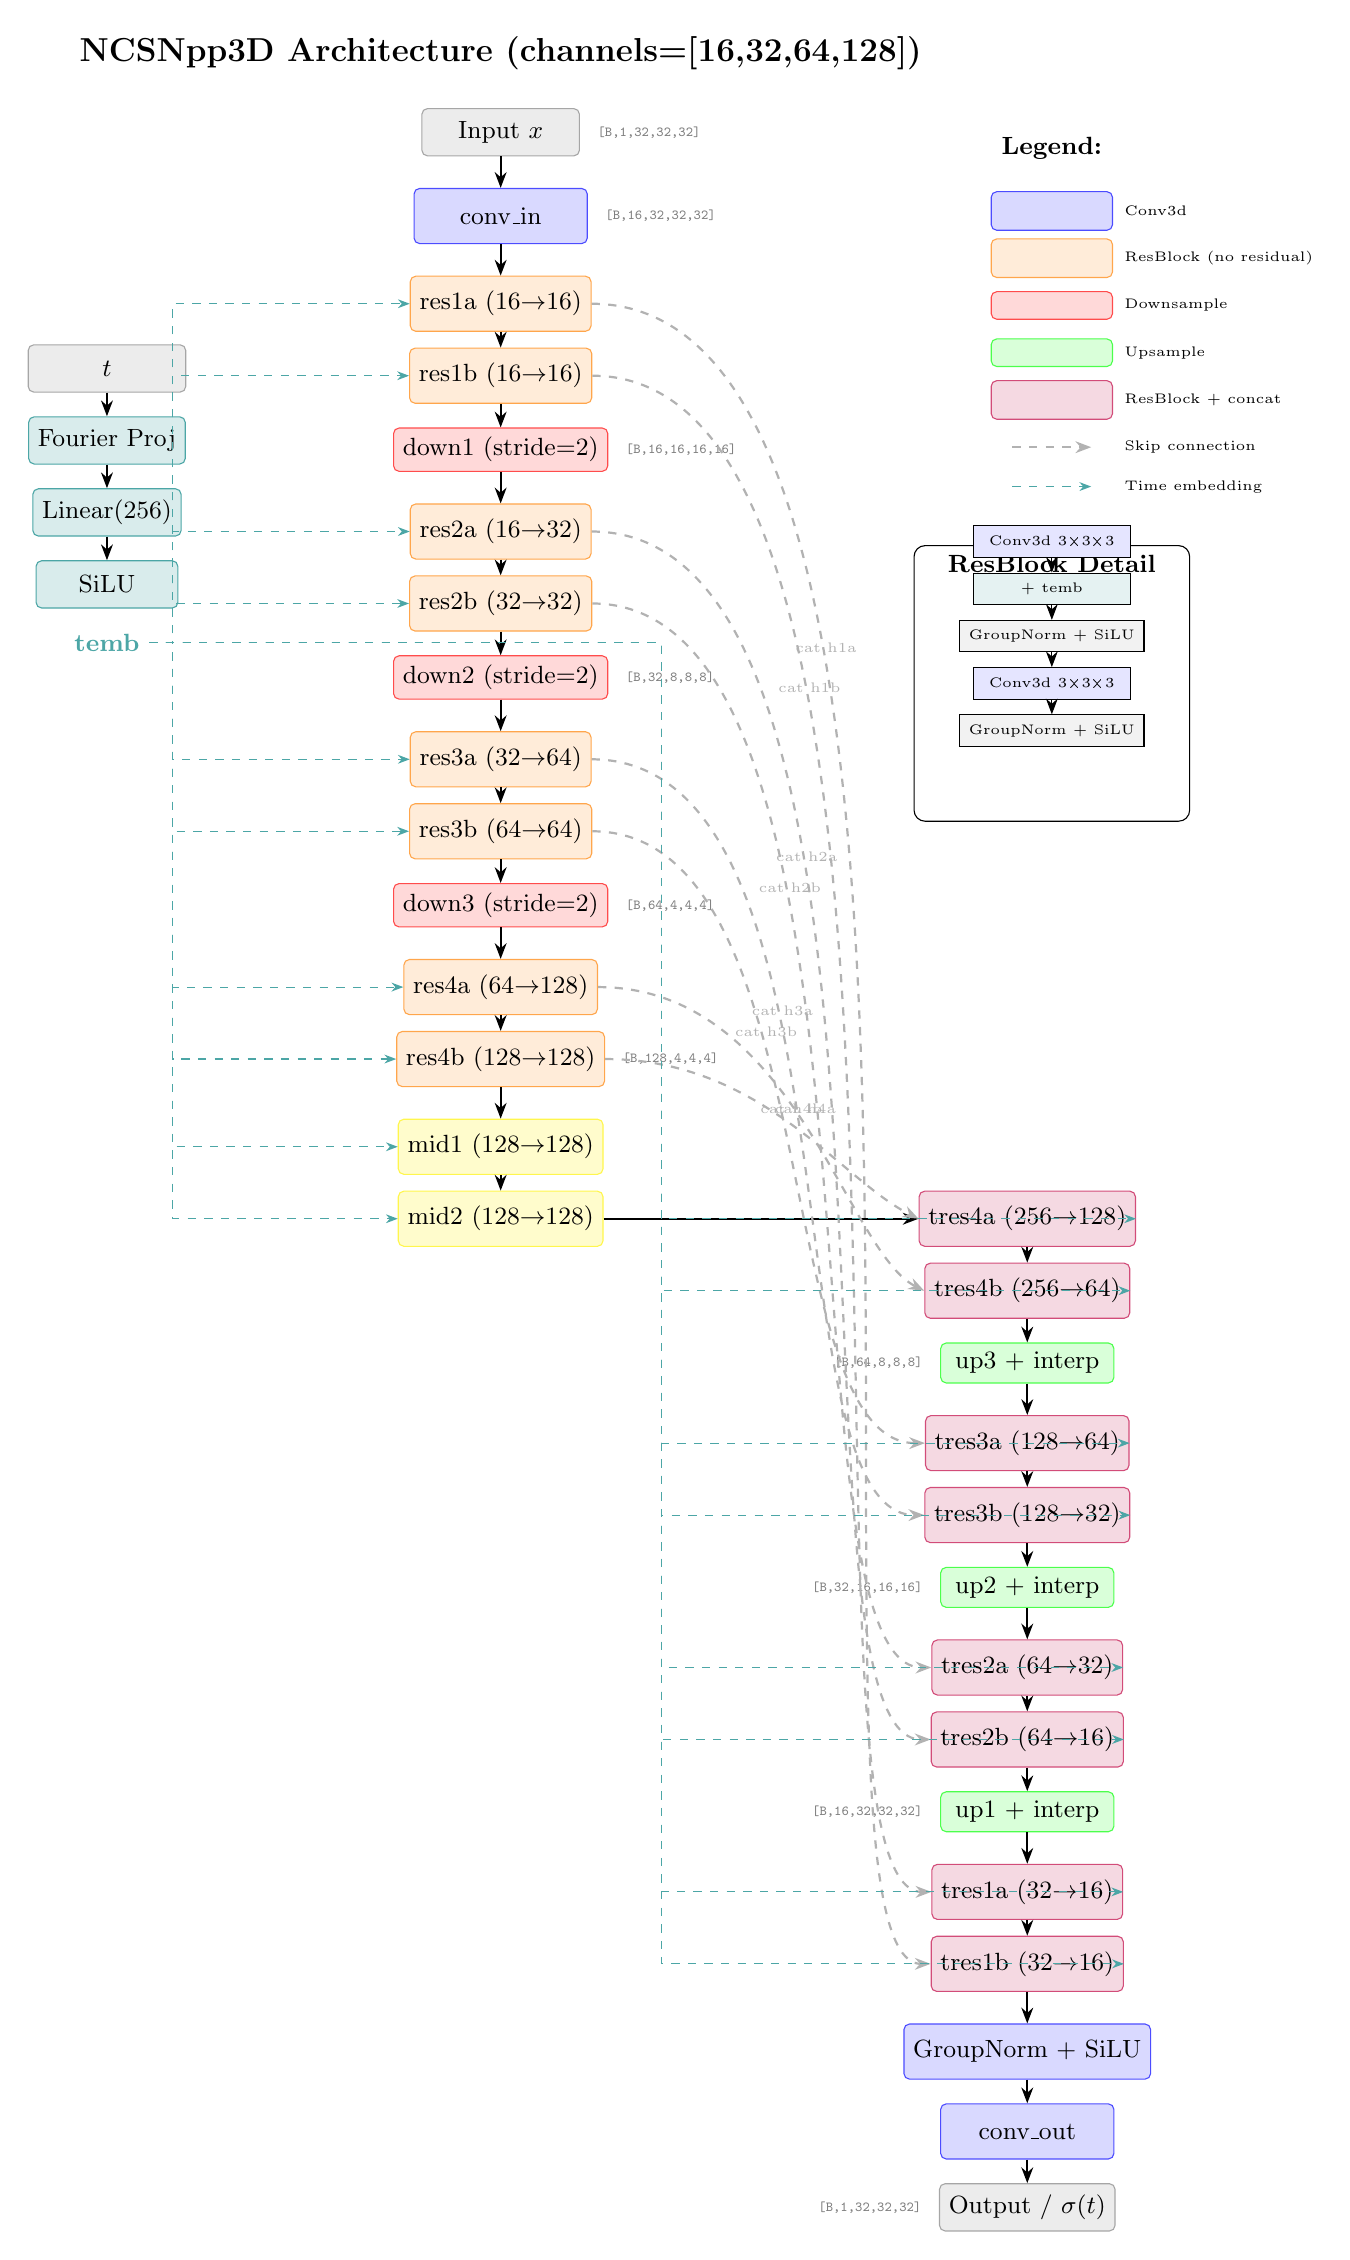
\begin{tikzpicture}[
    % Styles
    convblock/.style={rectangle, draw=blue!70, fill=blue!15, minimum width=2.2cm, minimum height=0.7cm, rounded corners=2pt, font=\small},
    resblock/.style={rectangle, draw=orange!70, fill=orange!15, minimum width=2.2cm, minimum height=0.7cm, rounded corners=2pt, font=\small},
    downblock/.style={rectangle, draw=red!70, fill=red!15, minimum width=2.2cm, minimum height=0.5cm, rounded corners=2pt, font=\small},
    upblock/.style={rectangle, draw=green!70, fill=green!15, minimum width=2.2cm, minimum height=0.5cm, rounded corners=2pt, font=\small},
    catblock/.style={rectangle, draw=purple!70, fill=purple!15, minimum width=2.2cm, minimum height=0.7cm, rounded corners=2pt, font=\small},
    embedblock/.style={rectangle, draw=teal!70, fill=teal!15, minimum width=1.8cm, minimum height=0.6cm, rounded corners=2pt, font=\small},
    ioblock/.style={rectangle, draw=gray!70, fill=gray!15, minimum width=2cm, minimum height=0.6cm, rounded corners=2pt, font=\small},
    arrow/.style={-{Stealth[length=2mm]}, thick},
    skiparrow/.style={-{Stealth[length=2mm]}, thick, dashed, gray!60},
    tembarrow/.style={-{Stealth[length=1.5mm]}, thin, teal!70, dashed},
    sizelabel/.style={font=\tiny\ttfamily, text=gray},
]

% Title
\node[font=\large\bfseries] at (0, 11) {NCSNpp3D Architecture (channels=[16,32,64,128])};

% Time embedding (left side)
\node[ioblock] (t_input) at (-5, 7) {$t$};
\node[embedblock, below=0.3cm of t_input] (fourier) {Fourier Proj};
\node[embedblock, below=0.3cm of fourier] (linear_emb) {Linear(256)};
\node[embedblock, below=0.3cm of linear_emb] (silu_emb) {SiLU};
\node[below=0.2cm of silu_emb, font=\small\bfseries, teal!70] (temb_label) {temb};

\draw[arrow] (t_input) -- (fourier);
\draw[arrow] (fourier) -- (linear_emb);
\draw[arrow] (linear_emb) -- (silu_emb);

% Input
\node[ioblock] (input) at (0, 10) {Input $x$};
\node[sizelabel, right=0.1cm of input] {[B,1,32,32,32]};

% Encoder (left column)
\node[convblock, below=0.4cm of input] (conv_in) {conv\_in};
\node[sizelabel, right=0.1cm of conv_in] {[B,16,32,32,32]};

\node[resblock, below=0.4cm of conv_in] (res1a) {res1a (16$\to$16)};
\node[resblock, below=0.2cm of res1a] (res1b) {res1b (16$\to$16)};
\node[downblock, below=0.3cm of res1b] (down1) {down1 (stride=2)};
\node[sizelabel, right=0.1cm of down1] {[B,16,16,16,16]};

\node[resblock, below=0.4cm of down1] (res2a) {res2a (16$\to$32)};
\node[resblock, below=0.2cm of res2a] (res2b) {res2b (32$\to$32)};
\node[downblock, below=0.3cm of res2b] (down2) {down2 (stride=2)};
\node[sizelabel, right=0.1cm of down2] {[B,32,8,8,8]};

\node[resblock, below=0.4cm of down2] (res3a) {res3a (32$\to$64)};
\node[resblock, below=0.2cm of res3a] (res3b) {res3b (64$\to$64)};
\node[downblock, below=0.3cm of res3b] (down3) {down3 (stride=2)};
\node[sizelabel, right=0.1cm of down3] {[B,64,4,4,4]};

\node[resblock, below=0.4cm of down3] (res4a) {res4a (64$\to$128)};
\node[resblock, below=0.2cm of res4a] (res4b) {res4b (128$\to$128)};
\node[sizelabel, right=0.1cm of res4b] {[B,128,4,4,4]};

% Middle
\node[resblock, below=0.4cm of res4b, fill=yellow!20, draw=yellow!70] (mid1) {mid1 (128$\to$128)};
\node[resblock, below=0.2cm of mid1, fill=yellow!20, draw=yellow!70] (mid2) {mid2 (128$\to$128)};

% Decoder (right column) - positioned to the right
\node[catblock, right=4cm of mid2] (tres4a) {tres4a (256$\to$128)};
\node[catblock, below=0.2cm of tres4a] (tres4b) {tres4b (256$\to$64)};
\node[upblock, below=0.3cm of tres4b] (up3) {up3 + interp};
\node[sizelabel, left=0.1cm of up3] {[B,64,8,8,8]};

\node[catblock, below=0.4cm of up3] (tres3a) {tres3a (128$\to$64)};
\node[catblock, below=0.2cm of tres3a] (tres3b) {tres3b (128$\to$32)};
\node[upblock, below=0.3cm of tres3b] (up2) {up2 + interp};
\node[sizelabel, left=0.1cm of up2] {[B,32,16,16,16]};

\node[catblock, below=0.4cm of up2] (tres2a) {tres2a (64$\to$32)};
\node[catblock, below=0.2cm of tres2a] (tres2b) {tres2b (64$\to$16)};
\node[upblock, below=0.3cm of tres2b] (up1) {up1 + interp};
\node[sizelabel, left=0.1cm of up1] {[B,16,32,32,32]};

\node[catblock, below=0.4cm of up1] (tres1a) {tres1a (32$\to$16)};
\node[catblock, below=0.2cm of tres1a] (tres1b) {tres1b (32$\to$16)};

% Output
\node[convblock, below=0.4cm of tres1b] (norm_out) {GroupNorm + SiLU};
\node[convblock, below=0.3cm of norm_out] (conv_out) {conv\_out};
\node[ioblock, below=0.3cm of conv_out] (output) {Output / $\sigma(t)$};
\node[sizelabel, left=0.1cm of output] {[B,1,32,32,32]};

% Encoder arrows
\draw[arrow] (input) -- (conv_in);
\draw[arrow] (conv_in) -- (res1a);
\draw[arrow] (res1a) -- (res1b);
\draw[arrow] (res1b) -- (down1);
\draw[arrow] (down1) -- (res2a);
\draw[arrow] (res2a) -- (res2b);
\draw[arrow] (res2b) -- (down2);
\draw[arrow] (down2) -- (res3a);
\draw[arrow] (res3a) -- (res3b);
\draw[arrow] (res3b) -- (down3);
\draw[arrow] (down3) -- (res4a);
\draw[arrow] (res4a) -- (res4b);
\draw[arrow] (res4b) -- (mid1);
\draw[arrow] (mid1) -- (mid2);

% Middle to decoder
\draw[arrow] (mid2.east) -- ++(1,0) |- (tres4a.west);

% Decoder arrows
\draw[arrow] (tres4a) -- (tres4b);
\draw[arrow] (tres4b) -- (up3);
\draw[arrow] (up3) -- (tres3a);
\draw[arrow] (tres3a) -- (tres3b);
\draw[arrow] (tres3b) -- (up2);
\draw[arrow] (up2) -- (tres2a);
\draw[arrow] (tres2a) -- (tres2b);
\draw[arrow] (tres2b) -- (up1);
\draw[arrow] (up1) -- (tres1a);
\draw[arrow] (tres1a) -- (tres1b);
\draw[arrow] (tres1b) -- (norm_out);
\draw[arrow] (norm_out) -- (conv_out);
\draw[arrow] (conv_out) -- (output);

% Skip connections (curved)
\draw[skiparrow] (res4b.east) .. controls ++(2,0) and ++(-1,0.5) .. (tres4a.west) node[midway, above, font=\tiny] {cat h4b};
\draw[skiparrow] (res4a.east) .. controls ++(2.5,0) and ++(-1,0.5) .. (tres4b.west) node[midway, above, font=\tiny] {cat h4a};

\draw[skiparrow] (res3b.east) .. controls ++(3,0) and ++(-2,0) .. (tres3a.west) node[pos=0.4, above, font=\tiny] {cat h3b};
\draw[skiparrow] (res3a.east) .. controls ++(3.5,0) and ++(-2,0) .. (tres3b.west) node[pos=0.4, above, font=\tiny] {cat h3a};

\draw[skiparrow] (res2b.east) .. controls ++(4,0) and ++(-2,0) .. (tres2a.west) node[pos=0.35, above, font=\tiny] {cat h2b};
\draw[skiparrow] (res2a.east) .. controls ++(4.5,0) and ++(-2,0) .. (tres2b.west) node[pos=0.35, above, font=\tiny] {cat h2a};

\draw[skiparrow] (res1b.east) .. controls ++(5,0) and ++(-2,0) .. (tres1a.west) node[pos=0.3, above, font=\tiny] {cat h1b};
\draw[skiparrow] (res1a.east) .. controls ++(5.5,0) and ++(-2,0) .. (tres1b.west) node[pos=0.3, above, font=\tiny] {cat h1a};

% Time embedding connections (to all ResBlocks)
\foreach \block in {res1a, res1b, res2a, res2b, res3a, res3b, res4a, res4b, mid1, mid2} {
    \draw[tembarrow] (temb_label.east) -- ++(.3,0) |- (\block.west);
}
\foreach \block in {tres4a, tres4b, tres3a, tres3b, tres2a, tres2b, tres1a, tres1b} {
    \draw[tembarrow] (temb_label.east) -- ++(6.5,0) |- (\block.east);
}

% Legend
\begin{scope}[shift={(7, 9)}]
    \node[font=\small\bfseries] at (0, 0.8) {Legend:};
    \node[convblock, scale=0.7] at (0, 0) {};
    \node[right, font=\tiny] at (0.8, 0) {Conv3d};
    \node[resblock, scale=0.7] at (0, -0.6) {};
    \node[right, font=\tiny] at (0.8, -0.6) {ResBlock (no residual)};
    \node[downblock, scale=0.7] at (0, -1.2) {};
    \node[right, font=\tiny] at (0.8, -1.2) {Downsample};
    \node[upblock, scale=0.7] at (0, -1.8) {};
    \node[right, font=\tiny] at (0.8, -1.8) {Upsample};
    \node[catblock, scale=0.7] at (0, -2.4) {};
    \node[right, font=\tiny] at (0.8, -2.4) {ResBlock + concat};
    \draw[skiparrow] (-0.5, -3) -- (0.5, -3);
    \node[right, font=\tiny] at (0.8, -3) {Skip connection};
    \draw[tembarrow] (-0.5, -3.5) -- (0.5, -3.5);
    \node[right, font=\tiny] at (0.8, -3.5) {Time embedding};
\end{scope}

% ResBlock detail box
\begin{scope}[shift={(7, 3)}]
    \node[draw, rounded corners, fill=white, minimum width=3.5cm, minimum height=3.5cm] (resbox) {};
    \node[font=\small\bfseries, anchor=north] at (resbox.north) {ResBlock Detail};
    \node[rectangle, draw, fill=blue!10, minimum width=2cm, minimum height=0.4cm, font=\tiny] (c1) at (0, 1.8) {Conv3d 3×3×3};
    \node[rectangle, draw, fill=teal!10, minimum width=2cm, minimum height=0.4cm, font=\tiny] (add) at (0, 1.2) {+ temb};
    \node[rectangle, draw, fill=gray!10, minimum width=2cm, minimum height=0.4cm, font=\tiny] (gn1) at (0, 0.6) {GroupNorm + SiLU};
    \node[rectangle, draw, fill=blue!10, minimum width=2cm, minimum height=0.4cm, font=\tiny] (c2) at (0, 0) {Conv3d 3×3×3};
    \node[rectangle, draw, fill=gray!10, minimum width=2cm, minimum height=0.4cm, font=\tiny] (gn2) at (0, -0.6) {GroupNorm + SiLU};
    \draw[arrow, thin] (c1) -- (add);
    \draw[arrow, thin] (add) -- (gn1);
    \draw[arrow, thin] (gn1) -- (c2);
    \draw[arrow, thin] (c2) -- (gn2);
\end{scope}

\end{tikzpicture}
\end{document}
